%
\chapter[Hints and Solutions]{Hints and Solutions for Selected Exercises}

\noindent
\emph{``In the book of life, the answers aren't in the back.''}

\hfill        -- Charlie Brown (Charles Schulz)

\bigskip
\textbf{\ref{ex:UnconstrPopGrowth_halflife_formula}} $\ds r = \frac{\ln 2}{h}$

\medskip
\textbf{\ref{ex:UnconstrPopGrowth_americium}}
Let $y(t)$ be the amount of americium-241
(in mg) at time $t$ (in years). Then
\[
   y(t) = 3e^{\frac{(\ln 2)t}{458}}
\]
\begin{enumerate}
\item[(a)] $y(10) \approx 2.9549$ mg.
\item[(b)] $y(916) = 0.75$ mg. (Note that 916 is two halflives, so $y(916)$
is one quarter of the initial amount.)
\item[(c)] $y(10000) \approx 8.0244\times 10^{-7}$ mg.
\end{enumerate}

\medskip
\textbf{\ref{ex:NewtonsLawOfCooling}}
Let $t$ be time;
let $h(t)$ be the temperature of the object
at time $t$;
let $A$ be the ambient temperature;
and let $k$ be the proportionality constant in
Newton's Law of Cooling.
Then, since ``\emph{the rate of change of the temperature of the
object}'' is $\frac{dh}{dt}$, and ``\emph{the difference
between the temperature of the object and the ambient
temperature}'' is $h-A$, the differential equation is
\[
   \frac{dh}{dt} = - k (h-A).
\]
The minus sign is necessary for the equation to agree with
our physical intuition: if $h>A$, the object is warmer than the ambient
temperature, and it should cool off. This means $h(t)$ should
decrease, so $\frac{dh}{dt}$ must be negative.  We assumed
$k>0$, so the equation requires the minus sign.


\medskip
\textbf{\ref{ex:AutFirstOrder_autclassify}}
\begin{tabbing}
\hspace*{0.25in} \= \hspace*{1.5in} \= \hspace*{1.5in} \= \kill
~ \> 
(a) autonomous \>
(b) nonautonomous \>
(c) nonautonomous \\[2pt]
~ \>
(d) nonautonomous \>
(e) autonomous \>
(f) autonomous
\end{tabbing}

\medskip
\textbf{\ref{ex:AutonomousDegreeThree}}
\begin{enumerate}
\item[(a)]
Let $f(y) = (y-2)(y^2+6y+8)$.
To find the equilibrium solutions, we must solve
$f(y)=0$; that is,
\[
   (y-2)(y^2+6y+8) = 0.
\]
This polynomial factors as $(y-2)(y+2)(y+4)$, so the
equilibrium solutions are $y(t)=2$, $y(t)=-2$ and $y(t)=-4$.
The polynomial is a cubic, and the coefficient of $y^3$ is 1,
so we have: $f(y) < 0$ if $y < -4$;
$f(y) > 0$ if $-4 < y < -2$;
$f(y) < 0$ if $-2 < y < 2$; and
$f(y) > 0$ if $y > 2$.
The graph of $f(y)$ looks something like this:

\centerline{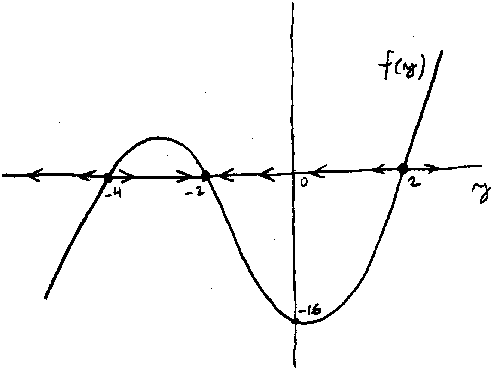
\includegraphics[width=4in]{images/AutonomousDegreeThreePlota.eps}}

The arrows on the $y$ axis indicate the whether
$y(t)$ is increasing or decreasing.
(This is the ``phase line'' for the differential equation.)

%\newpage
\item[(b)]
Here is a rough sketch of several solutions:

\centerline{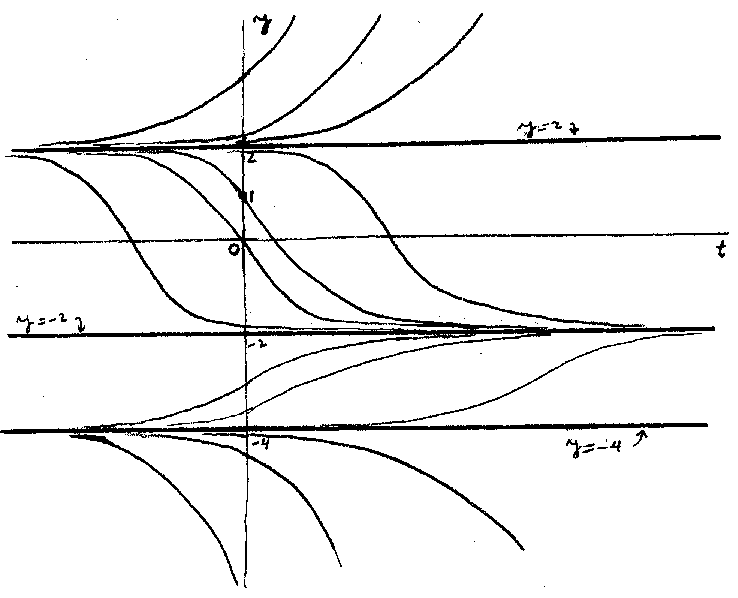
\includegraphics[width=4in]{images/AutonomousDegreeThreePlotb.eps}}

The horizontal lines $y=-4$, $y=-2$ and $y=2$ are the
equilibrium solutions.  The other curves
(not including the axes, of course) are rough sketches
of additional solutions.
Each solution has a different initial condition.
\item[(c)]
If $y(0)=1$, then $\ds \lim_{t\rightarrow\infty} y(t) = -2$
and $\ds \lim_{t\rightarrow -\infty} y(t) = 2$.
A rough sketch of this solution is included above.
\end{enumerate}

\medskip
\textbf{\ref{ex:SolveFirstOrderYCubed}}
This equation is separable.  Separating gives
\[
   y^{-3}dy = dt,
\]
and integrating gives
\[
  -y^{-2}/2 = t + c.
\]
We use the initial condition $y(0)=-2$ to determine $c$.
We have
\[
  c = -(-2)^{-2}/2 = -1/8.
\]
Now solving for $y$ gives
\[
  y = \frac{1}{\pm\sqrt{-2t+1/4}}.
\]
Because of the $\pm$, this is actually two solutions, and we must again use
the initial condition to determine the sign.  Since we want $y(0)=-2$, we must
choose the negative sign.  The solution to the initial value problem is
\[
  y = \frac{-1}{\sqrt{-2t+1/4}}.
\]
(Note that this solution is only defined for $t < 1/8$.  The
solution has a vertical asymptote at $t=1/8$.)

\medskip
\textbf{\ref{ex:Nondim_lrgmP}}
There are two independent nondimensional parameters.
For example,
\[
   \pi_1 = \frac{g}{\ell r^2}, \quad \pi_2 = \frac{\ell P}{mr^2}
\]
(Other nondimensional parameters are possible, but there
must still be just two independent nondimensional parameters.)


\newpage
%\medskip
\textbf{\ref{ex:lanchester_ants}}
\begin{enumerate}
\item[(a)] Since $\alpha = 3\beta$, $\alpha > \beta$.
We are told that the black ants are larger and stronger than
the red ants, so the size of the black colony must be $y$,
and the size of the red colony is $x$.
\item[(b)] We have
\[
   \beta x^2 - 3\beta y^2 = \beta x_0^2 -3\beta y_0^2.
\]
We see that we can divide by $\beta$ on both sides.
Putting in the initial sizes of the colonies gives
\[
   x^2-3y^2 = (50000)^2-3(35000)^2 < 0.
\]
The right side is negative, so the curve must cross the $y$
axis. This means the black colony will win.
  When $x=0$, we find
\[
  y = \sqrt{\frac{3(35000)^2-(50000)^2}{3}} \approx 20000.
\]
So there will be approximately $20,000$ ants remaining in
the black colony.
\end{enumerate}

\textbf{\ref{ex:lanchester_general}}
The equation that we will use is \eqref{eqn:lanchester_hyperbola}.
With $\alpha=\beta$,
we can cancel these constants to obtain
\[
   x^2 - y^2 = x_0^2 - y_0^2
\]
\begin{enumerate}
\item[(a)]
We first determine the results of the battles between the general's
5000 reinforcements and the opposing army's 2000 reinforcements.
We have $x_0=5000$ and $y_0=2000$.
Since $5000^2 - 2000^2 > 0$, the hyperbola crosses the $x$
axis.  We find the size of the surviving army by finding this
$x$-intercept (where $y=0$):
\[
   x = \sqrt{5000^2-2000^2} \approx 4582
\]
This is the number of reinforcements that survive to join
the general's main army of 6500, resulting in a total
of 11082 in the general's army.

We now have a battle with $x_0 = 11082$ and $y_0 = 10000$.
The general
will again win, and the size of his army after the main battle
will be
\[
   x = \sqrt{11082^2 - 10000^2} \approx 4776.
\]
\item[(b)]
If the main battle begins before the general's reinforcements arrive,
the sizes of the armies remain on the curve
\[
   x^2 - y^2 = 6500^2 - 10000^2.
\]
Since the line $y=x$ is the set of initial conditions
that lead to mutual annihilation, the latest that the 
reinforcements can arrive is when the coordinates of a point
on the above hyperbola are such that $x+4582 = y$.
That is,
\[
   x^2- (x+4582)^2 = 6500^2 - 10000^2
\]
which we solve for $x$ to find
\[
   x \approx 4011
\]
If the general's army falls below this size before the
reinforcements arrive, he will still lose the battle.
The question actually asked for the losses that the
general could sustain and still win the battle
when the reinforcements arrive, so the final answer
to this question is $6500-4011 = 2489$.
\end{enumerate}
%
%
\newpage
%
%\medskip
\textbf{\ref{ex:regmarkov1}}
\begin{enumerate}
\item[(a)] The transition diagram:

\medskip
\centerline{%
\includegraphics[width=4in]{fig/MarkovProbSol.eps}
}
\medskip

\item[(b)]
We find
\[
  A^2= \begin{bmatrix}
           \frac{363}{400} & \frac{37}{200} & \frac{37}{200} \T\B \\
	   \frac{19}{400} & \frac{1}{200}   & \frac{1}{200} \B  \\
	   \frac{9}{200}    & \frac{81}{100} & \frac{81}{100} \B
      \end{bmatrix}
\]
Since each entry in $A^2$ is positive, the Markov chain is regular.
\item[(c)]
To find the long-term probability distribution, we find an eigenvector
associated with the eigenvalue $\lambda=1$, and normalize it so that
it is a probability vector.
Thus, we must solve
\[
  (A-I)\BW = \BZero.
\]
We form the augmented matrix,
and then reduce it to reduced row echelon form:
\[
\begin{bmatrix}
   -1/20 & 1/10 & 1/10 & \vdots & 0 \\
   1/20  &   -1  &  0   & \vdots & 0 \\
   0     &  9/10 & -1/10 & \vdots & 0
\end{bmatrix}
\rightarrow
\begin{bmatrix}
   1  &   0  & -20/9  & \vdots & 0 \\
   0  &   1  & -1/9   & \vdots & 0 \\
   0  &   0  &  0     & \vdots & 0
\end{bmatrix}
\]
The third component $w_3$ of $\BW$ is arbitrary, so we may write
the set of solutions as
\[
   \BW = w_3 \begin{bmatrix}
               \frac{20}{9} \T\B \\ \frac{1}{9} \B\\ 1
             \end{bmatrix} .
\]
For $\BW$ to be a probability vector, we must have $w_1+w_2+w_3=1$,
which implies $w_3 = 9/30$.  Then the long-term probability vector
is
\[
  \BW = \begin{bmatrix}
          \frac{2}{3} \T\B \\ \frac{1}{30} \B \\ \frac{3}{10} \B
        \end{bmatrix} .
\]
\end{enumerate}

% \newpage
\textbf{\ref{ex:regmarkov2}}
\begin{enumerate}
\item[(a)] The transition matrix is
\[
  A = \begin{bmatrix}
           \frac{1}{4}  & \frac{1}{2} & 1 \T\B \\
	   \frac{1}{4}  & \frac{1}{2} & 0 \B \\
	   \frac{1}{2}  & 0   & 0 \B
      \end{bmatrix}
\]
Then
\[
  A^2 = \begin{bmatrix}
           \frac{11}{16}  & \frac{3}{8} & \frac{1}{4} \T\B \\
	   \frac{3}{16}  & \frac{3}{8} & \frac{1}{4} \B \\
	   \frac{1}{8}  & \frac{1}{4}   & \frac{1}{2} \B
      \end{bmatrix}
\]
and since each entry in $A^2$ is positive, the Markov chain
is regular.
\item[(b)]  As in the previous problem, we must find the probability
vector $\BW$ such that $(A-I)\BW=\BZero$.
By following the same steps as before, we find
\[
   \BW = \begin{bmatrix}
            \frac{1}{2} \T\B \\ \frac{1}{4} \B \\ \frac{1}{4} \B \\
         \end{bmatrix}
\]
Thus, in the long run, the probabilities of being in state A, B or C
are $1/2$, $1/4$ and $1/4$, respectively.
\end{enumerate}

\textbf{\ref{ex:regmarkov3}}
The transition matrix is
\begin{equation}
 A = \begin{bmatrix}
        0.6 & 0.4 & 0.2   \\
        0.2 & 0.5 & 0.2   \\
        0.2 & 0.1 & 0.6
     \end{bmatrix}
\end{equation}
An eigenvector associated with the eigenvalue $\lambda=1$
is $[3/2 \quad 1 \quad 1]^{\textsf{T}}$, and we divide by $7/2$ to create
the probability vector
\[
   \BW = \begin{bmatrix} 3/7 \\ 2/7 \\ 2/7 \end{bmatrix}
\]
This vector gives the long-term probability distribution
of the Markov chain.
Thus, in the long-term, we expected $3/7$ of the males to
be farmers, $2/7$ laborers, and $2/7$ professionals.

\medskip
\textbf{\ref{ex:markov3}}
The transition diagram for this version of the Coin and Die game is

\medskip
\centerline{%
\includegraphics[width=3.5in]{fig/ModCoinAndDieStateDiagram.eps}
}
and the transition matrix is
\[
A = \begin{bmatrix}
        1  &  0  & \frac{1}{2} & 0 \T \B \\
	0  &  1  &   0         & \frac{1}{3} \B \\
	0  &  0  &   0         & \frac{1}{2} \B \\
	0  &  0  & \frac{1}{2} & \frac{1}{6} \B \\
    \end{bmatrix}
\]
So
\[
  R = \begin{bmatrix}
          \frac{1}{2} & 0 \T\B \\
	      0       & \frac{1}{3} \B 
      \end{bmatrix}
  \quad \textrm{and}\quad
  Q = \begin{bmatrix}
          0 & \frac{1}{2} \T\B \\
	  \frac{1}{2}    & \frac{1}{6} \B 
      \end{bmatrix}
\]
and we calculate
\[
I-Q = \begin{bmatrix}
          1 & -\frac{1}{2} \T\B \\
	  -\frac{1}{2}    & \frac{5}{6} \B 
      \end{bmatrix},
 \quad
N = (I-Q)^{-1} =
      \begin{bmatrix}
          \frac{10}{7} & \frac{6}{7} \T\B \\
	  \frac{6}{7}  & \frac{12}{7} \B 
      \end{bmatrix},
\]
and
\[
B = R(I-Q)^{-1} =
      \begin{bmatrix}
          \frac{5}{7} & \frac{3}{7} \T\B \\
	  \frac{2}{7}  & \frac{4}{7} \B 
      \end{bmatrix}.
\]
With $N$ and $B$, we can answer the questions.
\begin{enumerate}
\item[(a)] If \emph{Coin} goes first, the expected number
of turns is the sum of the entries in the first column
of $N$, which is $\frac{16}{7} \approx 2.29$.
The probability that \emph{Coin} wins if \emph{Coin}
goes first is given by the entry in the first
row and column of $B$, which is
$\frac{5}{7} \approx 0.714$.
\item[(b)] If \emph{Die} goes first, the expected number
of turns is the sum of the entries in the second column
of $N$, which is $\frac{18}{7} \approx 2.57$.
The probability that \emph{Coin} wins if \emph{Die}
goes first is given by the entry in the first
row and second column of $B$, which is
$\frac{3}{7} \approx 0.429$.
\end{enumerate}
